\question{4}{4} Answer the following questions.

\begin{subparts}
  \item The figures below are formed by dots. Write down the number of dots in the 5th and 6th figures.
  \par\noindent\hspace*{5em}%
    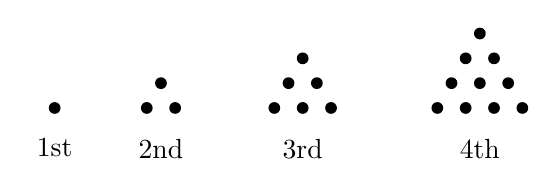
\begin{tikzpicture}[baseline=(current bounding box.center),scale=0.45,
      dot/.style={circle,fill,inner sep=1.5pt}]
      \foreach \x/\label in {0/1st,3/2nd,7/3rd,12/4th} {
        \node[below] at (\x,-0.6) {\label};
      }
      \node[dot] at (0,0) {};
      \foreach \x/\y in {2.6/0,3.4/0,3/0.7} {
        \node[dot] at (\x,\y) {};
      }
      \foreach \x/\y in {6.2/0,7/0,7.8/0,6.6/0.7,7.4/0.7,7/1.4} {
        \node[dot] at (\x,\y) {};
      }
      \foreach \x/\y in {10.8/0,11.6/0,12.4/0,13.2/0,11.2/0.7,12/0.7,12.8/0.7,11.6/1.4,12.4/1.4,12/2.1} {
        \node[dot] at (\x,\y) {};
      }
    \end{tikzpicture}
  \par

  \item A pattern is formed by sticks. The 1st pattern uses 6 sticks and each subsequent pattern uses 4 more sticks than the previous one. Write down the number of sticks in the 5th and 6th patterns.

  \item It is given that the $n$th term of a sequence is $8n+1$. Write down the 5th and 6th terms.

  \item Consider the sequence $3,\ -6,\ 12,\ -24,\ 48,\ \ldots$ Write down the next two terms.
\end{subparts}

\answerlines{14}
